%!TEX program = xelatex
\PassOptionsToPackage{quiet}{xeCJK}
\documentclass[hazy,blue,11pt]{elegantnote}
\title{PARTIAL DIFFERENTIAL EQUATIONS}

\author{{\CJKfontspec{SIMSUN.ttf} 姜嘉喆}}

\date{\zhtoday}

\usepackage{array}
\usepackage{mathrsfs} 


\begin{document}
    
\maketitle

\centerline{
  
\includegraphics[width=0.2\textwidth]{cat.png}
}
\section{数学专有词汇英文}

\subsection{Where PDEs come from}
\subsubsection{WHAT IS A PARTIAL DIFFERENTIAL EQUATION?}
    partial differential equation:偏微分方程

    differentiable:可微分
    
    boundary conditions:边界条件
    
    initial conditions:初始条件

    denote:表示

    subscripts:下标

    independent variables:自变量

    dependent variable:因变量

    derivatives:导数;partial derivatives:偏导数

    first order:一阶(偏导数)

    satisfies :满足

    equation:等式
    
    identically:相同

    region:区域

    reverses:颠倒

    separable ODE:可分离常微分方程

    distinguished:区别

    linear:线性

    operator:算子

    homogeneous linear equation:齐次线性方程

    given function:给定函数

    inhomogeneous linear equation:非齐次线性方程

    cubic term:立方项

    advantage:优势

    solutions:(方程的)解

    superposition principle:叠加原理

    vector spaces:向量空间

    exclusively:唯独

    constant coefficients:恒定系数

    arbitrary constants:任意常量

    integrate:整合

    integrable:可积的

    differentiating:求导数

    fixed:固定

    Geometrically:几何

    curve:曲线

    surface:曲面

    graph:图

    surface:曲面

    equally spaced:等间距

    value:值

    column:列

    multiple integrals:多重积分

    double integral:二重积分

    keep in mind:谨记

    exist and are continuous:存在且连续

    chain rule:链式法则

    integrals of derivatives:导数的积分

    Jacobians:雅可比(矩阵)

    Infinite series of functions :无穷级数

    Directional derivatives:方向导数

    tricky:棘手

\subsubsection{FIRST-ORDER LINEAR EQUATIONS}
    orthogonal:正交

    characteristic lines:特征线

    horizontal:水平

    auxiliary:辅助

    


\subsection{APPENDIX}    
\subsubsection{A.1 CONTINUOUS AND DIFFERENTIABLE FUNCTIONS}

    continuous:连续

    continuity:连续性
    
    closed interval:闭区间

    open interval:开区间

    half-open intervals:半开半闭区间

    symmetric interval:对称区间

    absolute value:绝对值

    endpoint:端点

    define:定义(。。。)

    intuitively:直观的

    Theorem:定理

    Intermediate:中间

    finite:有限

    x-axis:X轴

    rectangle:矩形

    encloses:包括

    contradicts:矛盾

    follows from:来自

    imply:意味着

    is said to:被称为

    discontinuity:间断

    piecewise:分段
    
    subinterval:子区间

    domains:域

    vector notation:矢量符号

    plane:平面

    domain:定义域,区域

    field:场(向量场)

    set:集合

    euclidean:欧式(distance)

    boundary point:边界点

    intersects:相交

    closure:闭包

    open set:开集

    close set:闭集

    bounded domain:有界域

    subdomains:子域

    analogous:类似
    (analog)
    
    indefinite integral:不定积分

    class:类

    positive integer:正整数

    gradient:梯度

    directional derivative:方向导数

    particle:(质)点

    It follows:它遵循

    scalar:标量

    coordinate:坐标

    coordinate systems:坐标系

    polar coordinates:极坐标

    cartesian coordinates:笛卡尔坐标

    matrix:矩阵

    determinant:行列式

    In case:以防

    In that case:在这种情况下

    with respect to:关于

    one-to-one:一对一

    curl-free:无卷曲

\subsubsection{INFINITE SERIES OF FUNCTIONS}

    series:级数

    infinite series:无穷级数

    series of functions:函数项级数

    geometric series:几何级数

    geometric series:等比级数

    power series:幂级数

    finite:有限

    partial sums:部分总和

    converge:收敛
    (convergence:收敛性)

    diverge:发散

    subtle example:微妙的例子
    (subtle): difficult to detect or analyze

    positive terms:正数项

    either A or B:或者A或者B

    contrapositive:逆否命题
    (逆命题: converse 否命题: inverse)

    comparison:比较

    ratio:比率

    deduction:推论

    pointwise:逐点(converges to f (x) pointwise)

    converges uniformly:一致收敛

    term by term:逐项

\subsubsection{DIFFERENTIATION AND INTEGRATION}

    differentiation:微分

    integration:积分

    general form:一般形式

    improper integrals:反常积分

    corollary:推论

    omit:省略

    multidimensional:多维的

    triple:三重

    parameterization:参数化(曲线的)

    parameter:参数(parametrization)

    semicircle:半圆

    counterclockwise:逆时针

    clockwise:顺时针

    parameter:参数

    partition:分割

    unit sphere:单位球面

    spherical coordinates:球面坐标

    overlap:重叠

    meet along:相交

    cube:立方体

    smooth faces:光滑面

    Alternatively:或者

    implicit function:隐函数

    spatial domain:空间域

    level set:水平集

    fundamental:基本集

    bounded plane domain:有界平面域

    bounded spatial domain:有界空间域

    traversed:遍历

    line integral:线积分

    unit tangent vector field:单位切向量场

    velocity field:速度场

    element:元素

    fluid:流体

    circulation:循环

    annulus:环

    equivalent:等价

    obtain:得到

    substitute:替换

    outwardpointing normal vector:向外(指向)法向量

    divergence:散度

    curl:旋度

    generalization:概括、推广

    origin:原点(0)

\subsubsection{DIFFERENTIAL EQUATIONS}

    initial condition:初始条件

    neighborhood:邻域

    singular point:奇异点
    (regular singular point:常规奇异点)

    quotient:商

    analytic:解析

    polynomials:多项式

    quadratic equation:二次方程

    convergent power series expansions:收敛幂级数扩展

    not differ by:不相差

    nonnegative:非负(整数)

\subsubsection{THE GAMMA FUNCTION}

    logarithm:对数

    exponential:指数

    factorial:阶乘

    properties:性质

    half-integers:半整数

    derivation:推导


\subsection{Waves and Diffusions}


\section{Where PDEs come from}
\subsection{WHAT IS A PARTIAL DIFFERENTIAL EQUATION?}
The define of PDE:written as $F(x,y,u(x,y),u_x(x,y),u_y(x,y))=F(x,y,u,u_x,u_y)=0)$ (first order), $x$,$y$ is some independent variable,$u(x,y)$ is an unknown function of these variables,$u_x(x,y),u_y(x,y)$ is the derivatives of $x$,$y$.\par
$F(x,y,u,u_x,u_y,u_{xx},u_{xy},u_{yy})=0)$(second order)

The solution of PDE: a function$u(x,y,...)$ that satisfies the equation identically, at least in some region of the $x, y, . . .$ variables.

Some examples of PDEs:\\
1.$u_x+u_y=0$(transport)\\
2.$u_x+yu_y=0$(transport)\\
3.$u_x+uu_y=0$(shock wave)\\
4.$u_{xx}+u_{yy}=0$(Laplace’s equation)\\
5.$u_tt-u_xx+u^3=0$(wave with interaction)\\
6.$u_t+uu_x+u_{xxx}=0$(dispersive wave)\\
7.$u_tt+u_{xxxx}=0$(vibrating bar)\\
8.$u_t-iu_{xx}=0$(quantum mechanics)

about order:Examples 1 to 3 have order one; 4, 5, and 8 have order two;\par
about linear:Examples 3,5 and 6 are not “linear.\par

\begin{note}
Linearity:$\mathscr{L}$ is an operator,The definition we want for linearity is 
\begin{equation}
   \mathscr{L}(u+v)=\mathscr{L}u+\mathscr{L}v,
   \mathscr{L}(cu)=c\mathscr{L}u
\end{equation}
for any functions $u$, $v$ and any constant $c$.$\mathscr{L}$ is called linear operator. The equation
\begin{equation}
    \mathscr{L}u=0
\end{equation}
s called a homogeneous linear equation. The equation
\begin{equation}
    \mathscr{L}u=g
\end{equation} is called an inhomogeneous linear equation.
     
\end{note}

\begin{theorem}[superposition principle]
    The advantage of linearity for the equation $\mathscr{L}u=0$ is that if $u$ and $v$ are both solutions, so is $(u+v)$. If $u_1,..., u_n$ are all solutions,so is any linear combination:
\begin{equation}
    c_1 u_1(x)+...+c_n u_n(x)=\sum_{j=1}^n c_j u_j(x)
\end{equation}
\end{theorem}
\begin{theorem}
    For an $ODE$ of order m, you get m arbitrary constants.
\end{theorem}

\begin{note}
    There are two arbitrary functions in the solution. Find all $u(x,y)$ satisfying the equation $u_xx=0$, we can integrate once to get $u_x$=constant. But that’s not really right since there is another variable $y$. What we really get is $u_x(x,y)=f(y)$, where $f(y)$ is arbitrary. Do it again to get $u(x,y)=f(y)x+g(y)$.
\end{note}

a few things to keep in mind:
\begin{enumerate}
  \item Derivatives are local
  \item Mixed derivatives are equal(in this book)
  \item The chain rule is used frequently in PDEs
  \item Integrals of derivatives:see Section A.3
  \item Derivatives of integrals:see Section A.3
  \item Jacobians (change of variable in a double integral):see Section A.1
  \item Infinite series of functions and their differentiation:see Section A.2
  \item Directional derivatives:see Section A.1
\end{enumerate}

\section{APPENDIX}%数分中学的东西
\subsection{A.1 CONTINUOUS AND DIFFERENTIABLE FUNCTIONS}
\begin{definition}[limit]
    The function $f(x)$ has the limit $L$ as $x$ approaches $a$ if for any number $\epsilon>0$ (no matter how small) there exists a number $\delta>0$ such that $0<|x-a|<\delta$ implies that $|f(x)-L|<\epsilon$ We write $\lim\limits_{x \to a} f(x) =L$.
\end{definition}

\begin{note}
    It doesn’t matter what the function is at $x = a$ itself;
    We can also define the one-sided limits,the only difference from the ordinary (two-sided) limit is the removal of the absolute value.
\end{note}

\begin{definition}[continuous]
    The function $f(x)$ is continuous at a point a if the limit of $f(x)$ as $x \to a$ exists and equals $f(a)$.
\end{definition}

\begin{note} 
~\\
\begin{enumerate}
    \item Compared with limit, the function has to be defined at a.
    \item A function is continuous in an interval $b \leq x \leq c$ if it is continuous at each point of that interval. Intuitively, the graph of a continuous function can be drawn without lifting the pen from the page.
    \item A function is said to have a jump discontinuity (or simply to have a jump) if both one-sided limits $f(x−)$ and $f(x+)$ exist (as finite numbers) but they are unequal.
    \item A function f(x) is called piecewise continuous on a finite closed interval $[a,b]$ if there are a finite number of points $a = a_0\le a_1\le \cdots \le a_n =b$ such that $f(x)$ is continuous on each open subinterval $(a_{j-1},a_j)$ and all the one-sided limits $f(a_{j}^{-})$ for $1 \le  j \le  n$ and $f(a_{j}^{+})$ for $0 \le j \le n−1$ exist.

\end{enumerate}   
\end{note}

\begin{theorem}[Intermediate Value Theorem]
    If $f(x)$ is continuous in a finite closed interval $[a,b]$, and $f(a) < p < f (b)$, then there exists at least one point $c$ in the interval such that $f(c)=p$.
\end{theorem}

\begin{theorem}[Theorem on the Maximum]
    If $f(x)$ is continuous in a finite closed interval $[a,b]$, then it has a maximum in that interval. That is, there is a point $m \in [a,b]$ such that $f (x) \leq f (m)$ for all $x \in [a, b]$.
\end{theorem}

\begin{theorem}[Vanishing Theorem]
    Let $f(x)$ be a continuous function in a finite closed interval $[a,b]$. Assume that $f(x) \ge 0$ in the interval and that $\int_{b}^{a} f(x)dx=0$. Then $f(x)$ is identically zero.
\end{theorem}

\begin{definition}[differentiable]
    A function $f(x)$ is differentiable at a point $a$ if the limit of $[f(x)-f(a)]/(x-a)$ as $x \to a$ exists. The value of the limit is denoted by ${f}'(a)$ or $\frac{\mathrm{d} f}{\mathrm{d} x}(a)$.
\end{definition}

\subsubsection{FUNCTIONS OF TWO OR MORE VARIABLES}
\begin{definition}[some points and field]
~\\
    \begin{enumerate}
        \item $domain or region$: an open set $D$(a set without its boundary).\\
                example:the ball $\left \{  \left | x-a \right |<R \right \}$ of center $a$ and radius $R$.
        \item $boundary point$: A boundary point of any set $D$ (in three-dimensional space) is a point $x$ for which every ball with center at $x$ intersects both $D$ and the complement of $D$.
        \item $bdy D$: the set of all boundary points of $D$.
        \item $open set$: it contains none of its boundary points.
        \item $closed set$: it contains all of its boundary points.
        \item $closure$: The $\overline{D}$ is the union of the domain and its boundary: $D=D \cup bdy D$.
    \end{enumerate}
\end{definition}

Some similar theorems to those for one variable:
\begin{theorem}[First Vanishing Theorem]
    Let $f(x)$ be a continuous function in $\overline{D}$ where $D$ is a bounded domain. Assume that $f(x) \ge 0$ in $\overline{D}$ and that $\iiint_{D}f(x)dx=0$, then f (x) is identically zero.
    \begin{note}
        A quantity which rigorously assumes the value of zero is said to be identically zero. The "identically" is used for emphasis when simply stating that a quantity is (or appears to be) zero is not considered sufficiently strong. A quantity that is identically zero is said to be vanishing, or sometimes (again for emphasis) to vanish identically.
    \end{note}
\end{theorem}

\begin{theorem}[Second Vanishing Theorem]
    Let $f(x)$ be a continuous function in $D_0$  such that $\iiint_{D}f(x)dx=0$ for all subdomains $D \subset D_0$. Then $f(x)\equiv 0$ in $D_0$.   
\end{theorem}

\begin{definition}[class $C^k$]
    A function is said to be of class $C^1$ in a domain $D$ if each of its partial
derivatives of first order exists and is continuous in $D$.If $k$ is any positive
integer, a function is said to be of class $C^k$ if each of its partial derivatives of order $\le k$ exists and is continuous.
\end{definition}

The mixed derivatives are equal(in this book), although pathological examples can be exhibited for which the mixed derivatives are not equal.
\begin{note}
    The term "pathological" is used in mathematics to refer to an example specifically cooked up to violate certain almost universally valid properties. Pathological problems often provide interesting examples of counterintuitive behavior, as well as serving as an excellent illustration of why very detailed conditions of applicability are required in order for many mathematical statements to be universally true.
\end{note}

The chain rule deals with functions of functions.

\begin{definition}[gradient]
    The gradient of a function (of three variables) is $\bigtriangledown f=(f_x,f_y,f_z)$.
\end{definition}

\begin{definition}[directional derivative]
    The directional derivative of $f(x)$ at a point $a$ in the direction of the vector $v$ is
    \begin{equation}
        \lim _{t \rightarrow 0} \frac{f(a+tv)-f(t)}t=v\cdot \nabla f(a)
    \end{equation}
\end{definition}

\subsubsection{VECTOR FIELDS}
A vector field assigns a vector to each point.
\begin{definition}[jacobian matrix]
    The first-order partial derivatives form a matrix
    \begin{equation}
        \mathscr{J}=\left(\begin{matrix}{\frac{\partial x}{\partial x^{\prime}}}&{\frac{\partial y}{\partial x^{\prime}}}\\ {\frac{\partial x}{\partial y^{\prime}}}&{\frac{\partial y}{\partial x^{\prime}}}\\ \end{matrix}\right),
    \end{equation}
    called the jacobian matrix
    The jacobian determinant is the determinant of this matrix, $J = det \mathscr{J}$.
\end{definition}

For example, the transformation from polar to cartesian coordinates $x=r\cos \theta , y=r\sin \theta $ has the jacobian matrix
\begin{equation}
    \mathscr{J}=\begin{pmatrix}\frac{\partial x}{\partial r}&\frac{\partial y}{\partial r}\\ \frac{\partial x}{\partial\theta}&\frac{\partial y}{\partial\theta}\end{pmatrix}=\begin{pmatrix}\cos\theta&\sin\theta\\ -r\sin\theta&r\cos\theta\end{pmatrix}.
    \nonumber
\end{equation}
The jacobian determinant is $J=\cos\theta\cdot r\cos\theta+\sin\theta\cdot r\sin\theta=r$.
Any change of coordinates in a multiple integral involves the jacobian. If
the transformation $x=g(x^{\prime},y^{\prime})$ and $y=h(x^{\prime},y^{\prime})$ carries the domain $D^{'}$ onto the domain $D$ in a one-to-one manner and is of class $C^1$, and if $f(x,y)$ is a continuous function defined on $\overline{D}$, then
\begin{equation}
    \iint\limits_D f(x,y)dxdy=\iint\limits_{D'}f(g(x',y'),h(x',y'))\cdot|U(x',y')|dx'dy'.
    \nonumber
\end{equation}
The size of the jacobian factor $\lvert J\rvert$ expresses the amount that areas are stretched or shrunk by the transformation. For example, a change to polar coordinates
gives $|J(x',y')|dx'dy'=rdrd\theta$.

\subsection{A.2 INFINITE SERIES OF FUNCTIONS}
\begin{definition}[some definitions]
~\\
    \begin{enumerate}
        \item infinite series: $\sum_{n=1}^{\infty}a_n$.
        \item partial sums: the sums of the first $N$ terms: $S_N=\sum_{n=1}^N a_n$.
        \item converge: if there is a finite number $S$ such that $\lim_{N \to \infty}S_N=S$. This means that for any number $\epsilon > 0$ (no matter how small) there exists an integer $\mathcal{N}$ such that $N \ge \mathcal{N}$ implies that $|S_N-S|<\epsilon$. $S$ is called the sum of the series.
        \item diverge: the series does not converge.
        \item absolutely convergent: If $\sum_{n=1}^{\infty}|a_{n}|$ converges, we say that $\sum_{n=1}^{\infty}a_{n}$ is absolutely convergent.
        \item conditionally convergent: If $\sum_{n=1}^{\infty}a_{n}$ converges but $\sum_{n=1}^{\infty}|a_{n}|$ diverges, we say that $\sum_{n=1}^{\infty}a_{n}$ is conditionally convergent.
        \begin{note}
            This book is full of conditionally convergent series.
        \end{note}
    \end{enumerate}    
\end{definition}

\begin{theorem}[Comparison Test]
    If  $\left|a_n\right| \le b_n$ for all $n$, and if $\sum_{n=1}^{\infty} b_n$ converges, then $\sum_{n=1}^{\infty} a_n$ converges absolutely. The contrapositive necessarily follows: If $\sum_{n=1}^{\infty}\left|a_n\right|$ diverges, so does $\sum_{n=1}^{\infty} b_n$. The limit comparison test states that if $a_n \ge 0$, $b_n \ge 0$, if $\lim _{n \rightarrow \infty} a_n / b_n=L$ where $0 \le L<\infty$, and if $\sum_{n=1}^{\infty} b_n$ converges, then so does $\sum_{n=1}^{\infty} a_n$.
\end{theorem}

\subsubsection{SERIES OF FUNCTIONS}
\begin{definition}[SERIES OF FUNCTIONS]
   Consider $\sum_{n=1}^{\infty}f_n(x)$, where $f_n(x)$ could be any functions.
\end{definition}
A simple example is the series 
\begin{equation}
    \sum\limits_{n=0}^{\infty}(-1)^{n}x^{2n}=1-x^2+x^4-x^6+\cdots,
\end{equation}
which we recognize as a geometric series with the ratio $-x^2$. The best
known series are the power series $\textstyle \sum_{n=1}^{\infty}(a_{n}x^{n})$, They have special convergence properties, such as convergence in a symmetric interval around $0$。
\begin{definition}[converges uniformly]
   We say that the series converges uniformly to $f(x)$ in $[a, b]$ if
\begin{equation}
    \max\limits_{a\le x\le b}\bigg|f(x)-\sum\limits_{n=1}^Nf_n(x)\bigg|\to0\quad\text{as}N\to\infty.
\end{equation}
\begin{note}
    收敛与一致收敛的关系及为啥用一致收敛,数分讲过了这里就不展开了。
\end{note}
\end{definition}

\begin{theorem}[Comparison Test]
   If $|f_n(x)| \le c_n$ for all $n$ and for all $a \le x \le b$, where
the $c_n$ are constants, and if $\sum_{n=1}^{\infty}c_n$ converges, then $\sum_{n=1}^{\infty}f_{n}(x)$ converges uniformly in the interval $[a, b]$, as well as absolutely.
\end{theorem}

\begin{theorem}[Convergence Theorem]
   If $\sum_{n=1}^\infty f_n(x) = f(x)$ uniformly in $[a,b]$ and if all the functions $f_n(x)$ are continuous in $[a,b]$, then the sum $f(x)$ is also continuous in $[a,b]$ and
\begin{equation}
    \sum\limits_{n=1}^\infty\int_a^b f_n(x)dx=\int_a^b f(x)dx.
\end{equation}
\end{theorem}

\begin{theorem}[Convergence of Derivatives]
  If all the functions $f_{n}(x)$ are differentiable in $[a,b]$ and if the series $\sum_{n=1}^{\infty}f_{n}(c)$ converges for some $c$, and if the series of derivatives $\sum_{n=1}^{\infty}f_n'(x)$ converges uniformly in $[a,b]$, then $\sum_{n=1}^{\infty}f_{n}(x)$ converges uniformly to a function $f(x)$ and
\begin{equation}
    \sum\limits_{n=1}f_n'(x)=f'(x).
\end{equation}
\end{theorem}

\subsection{A.3 DIFFERENTIATION AND INTEGRATION}
\subsubsection{DERIVATIVES OF INTEGRALS}
这块全是公式,直接截图过来吧。。。其实就是数分函数项级数那块的内容,一致收敛/连续后积分与微分可以交换顺序:

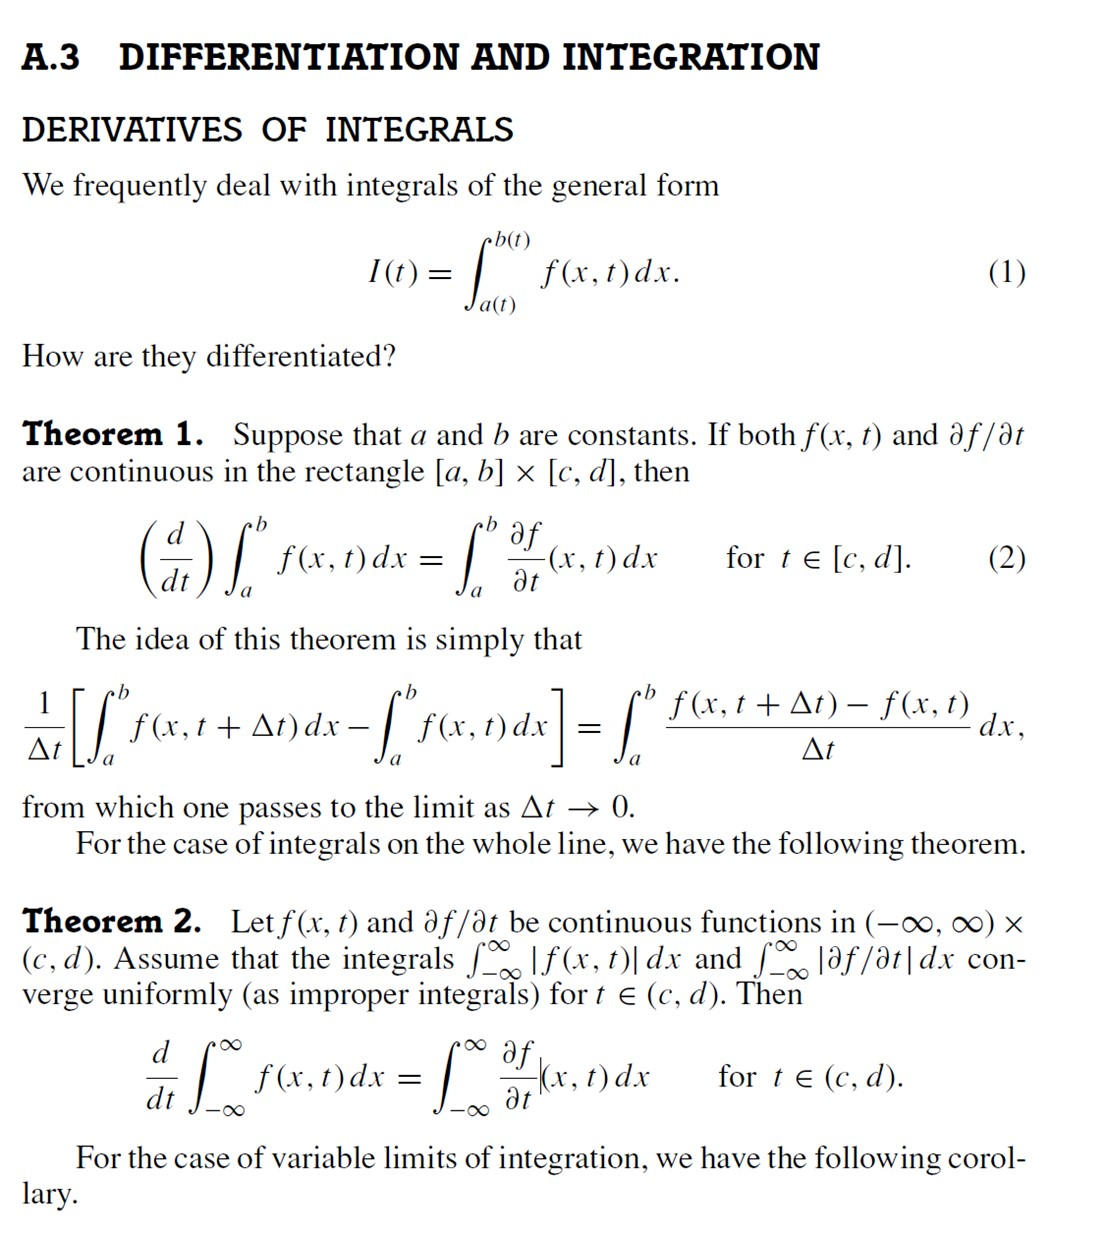
\includegraphics[width=\textwidth,keepaspectratio]
{image/A.3.1.jpg}

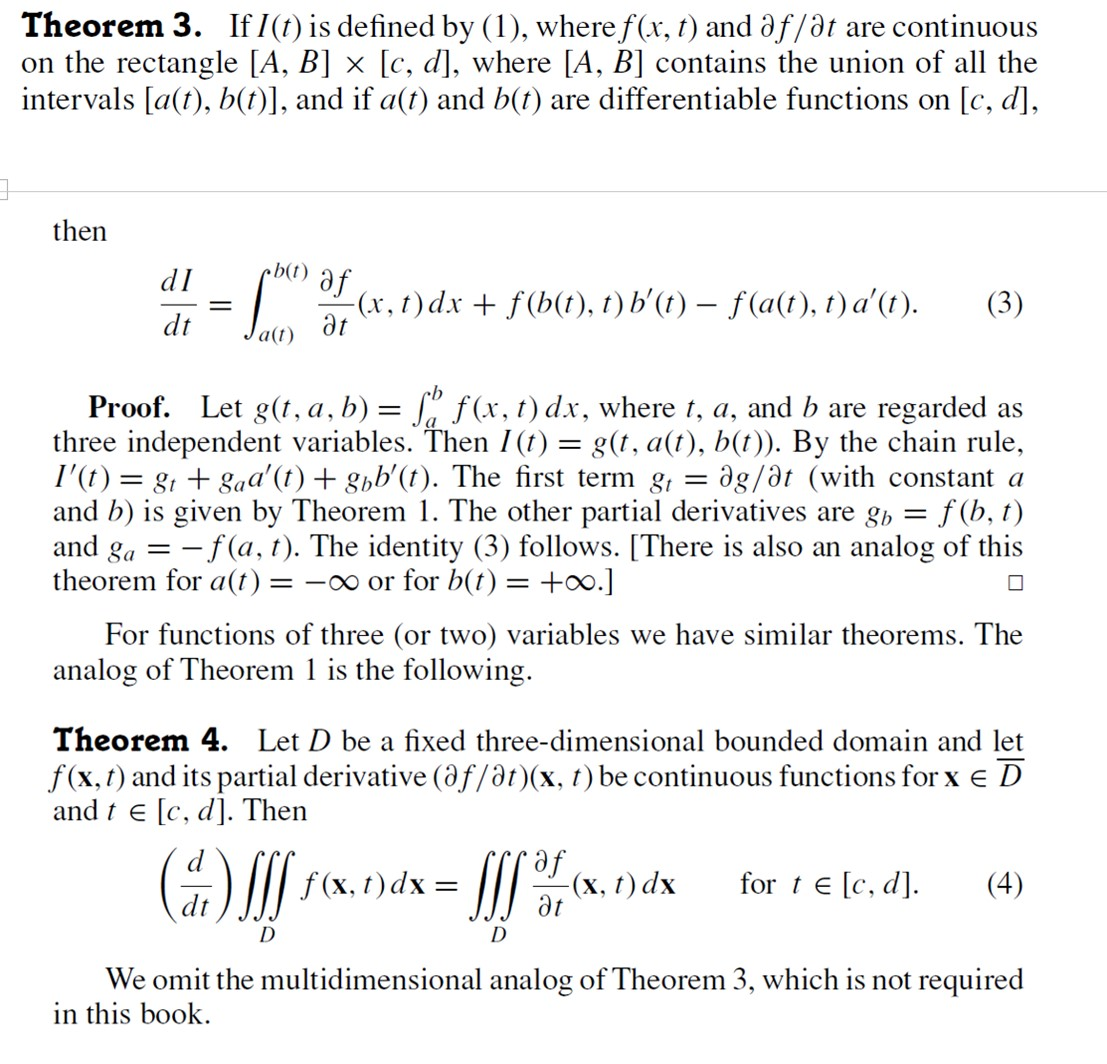
\includegraphics[width=\textwidth,keepaspectratio]
{image/A.3.2.jpg}

\subsubsection{CURVES AND SURFACES}
A curve may be intuitively visualized as the path continuously traced out by a
particle. More precisely, a curve $C$ in space is defined as a continuous function
from an interval $[a,b]$ into space. Thus it is given by a triple of continuous
functions
\begin{equation}
    x=f(t),\quad y=g(t),\quad z=h(t),\quad \text{for}a \leq t \leq b.
\end{equation}
The triple of functions is called a parameterization of the curve.If the three coordinate functions are of class $C^1$, we say that the curve $C$ is of class $C^1$.

A surface $S$ is defined as a continuous function from a closed set $\overline D$ in a plane into three-dimensional space. Thus it too is given by a triple of functions
\begin{equation}
    x=f(s,t),\quad y=g(s,t),\quad z=h(s,t)\quad\text{for}(s,t)\in\overline{D}.
\end{equation}
This triple of functions is a parametrization of $S$,the variables $s$ and $t$ are
the parameters, and $\overline D$ is the parameter domain. It is the image of the functions in three-dimensional space which corresponds to our intuitive notion of a surface.

A surface is of class $C^1$ if all three coordinate functions are of class $C^1$.The union of a finite number of overlapping surface is also considered to be a surface.

\subsubsection{INTEGRALS OF DERIVATIVES}
Some fundamental theorem of calculus:
\begin{theorem}[Green’s Theorem]
    Let $D$ be a bounded plane domain with a piecewise $C^1$ boundary curve $C=bdyD$. Consider $C$ to be parametrized so that it is traversed once with $D$ on the left. Let $p(x,y)$ and $q(x,y)$ be any $C^1$ functions defined on $\overline{D}=D\cup C$. Then
\begin{equation}
    \iint\limits_D(q_x-p_y)dxdy=\int\limits_Cpdx+qdy.
\end{equation}
\end{theorem}

The line integral on the right side may also be written as $\int_C\left(p,q\right)\cdot\text{t}ds$, where $t$ is the unit tangent vector field along the curve and $ds$ is the element of arc length. If $(p,q)$ is the velocity field of a fluid flow, the line integral is the circulation of the flow.

A completely equivalent formulation of Green’s theorem is obtained by
substituting $p=-g$ and $q=+f$. If $f=(f,g)$ is any $C^1$ vector field in $\overline{D}$, then $\iint_D(f_x+g_y)dxdy=\int_C(-gdx+fdy)$. If $n$ is the unit outwardpointing normal vector on $C$, then $n=(+dy/ds,−dx/ds)$. Hence Green’s theorem takes the form
\begin{equation}
    \iint\limits_D \nabla\cdot fdxdy=\int\limits_C f\cdot nds,
\end{equation}
where $\nabla\cdot f = f_x + g_y$ denotes the divergence of $f$.

\begin{theorem}[Divergence Theorem]
    Let $D$ be a bounded spatial domain with a piecewise $C^1$ boundary surface $S$. Let $n$ be the unit outward normal vector on $S$. Let $f(x)$ be any $C^1$ vector field on $\overline{D} = D \cup S$. Then
\begin{equation}    \iiint\limits_D\nabla\cdot\textbf{f}d\textbf{x}=\iint\limits_S\textbf{f}\cdot\textbf{n}dS,
\end{equation}
where $\nabla\cdot\textbf{f}$ is the three-dimensional divergence of $\textbf{f}$ and $dS$ is the element of surface area on $S$.
\end{theorem}

\subsection{A.4 DIFFERENTIAL EQUATIONS}
\begin{theorem}[Existence Theorem for ODEs]
    Consider the system of $ODEs$
\begin{equation}
   \frac{d\mathbf{u}}{dt}=\mathbf{f}(t,\mathbf{u}) 
\end{equation}
together with the initial condition $\mathbf{u}(a)=\mathbf{b}$. Let $\mathbf{f}(t,\mathbf{u})$ be a vector function of a scalar variable $t$ and a vector variable $\mathbf{u}$ of class $C^1$ in a neighborhood of the point $(a,\mathbf{b})$. Here $\mathbf{u}=(u_{1},u_{2},\ldots,u_{N})$ and $\mathbf{f}=(f_{1},f_{2},\ldots,f_{N})$. Then there exists a unique solution $\mathbf{u}(t)$ of class $C^1$ for $t$ in some open interval containing $a$.
\end{theorem}

\subsubsection{REGULAR SINGULAR POINTS}
A linear second-order ODE has the form
\begin{equation}
    a(t)u^{''}+b(t)u^{'}+c(t)u=0.
\end{equation}
Its solutions form a two-dimensional vector space. A point where one of the coefficients is infinite or where $a(t) = 0$ is called a $singular point$. Suppose
that the point in question is $t = 0$. The origin is called a $regular singular point$
if the quotient $b(t)/a(t)$ behaves no worse than $t^{−1}$ and the quotient $c(t)/a(t)$ behaves no worse than $t^{−2}$ near $t = 0$.

\begin{definition}[Euler equation]
\begin{equation}
    u^{''} + \frac{\beta}{t}u^{'} + \frac{\gamma}{t^2}u = 0 
\end{equation}   
\end{definition}
\begin{note}
    Let $r$ and $s$ denote the two roots of the quadratic equation
\begin{equation}
    x(x-1)+\beta x+\gamma=0,
\end{equation}
known as the $indicial equation$. Then the solutions of the simple Euler equation are $Ct^r+Dt^s$ for arbitrary $C$ and $D$, except in the case $r=s$. The exponents $r$ and $s$ are called the $indices$.
\end{note}

\newtheorem*{Theorem}{Theorem}
\begin{Theorem}
~\\
\begin{enumerate}
    \item If $r$ and $s$ do not differ by an integer, then all the solutions of ~\ref{equ:linear second-order ODE} have the form
\begin{equation}
    Ct^r\sum_{n=0}^\infty p_n\big|t^n+Dt^s\sum\limits_{n=0}^\infty q_n t^n
\end{equation}
with arbitrary $C$ and $D$. (This includes the case that $r$ and $s$ are complex.)

    \item If $s - r$ is a nonnegative integer, then the solutions have the form
\begin{equation}
    Ct^r\sum\limits_{n=0}^\infty p_n t^n+(Cm\log t+D)t^s\sum\limits_{n=0}^\infty q_n t^n
\end{equation}
for some constant $m$ and with arbitrary constants $C$ and $D$. In case $r = s$, we have $m = 1$. All these series converge in at least a neighborhood of $t = 0$.
\end{enumerate}
\end{Theorem}

\subsection{A.5 THE GAMMA FUNCTION}
\begin{definition}[gamma function]
\begin{equation}
    \Gamma(x)=\int_0^\infty s^{x-1}e^{-s}ds\quad\text{for}0<x<\infty.
\end{equation}   
\end{definition}
The integral converges. It has the following properties.
\begin{equation}
\begin{gathered}
\Gamma(x+1) =x\Gamma(x).  \\
\Gamma(n+1) =n!\quad\text{if}n\text{is a positive integer.}  \\
\Gamma\left(\frac{1}{2}\right) =\sqrt{\pi}\text{.}  
\end{gathered}
\end{equation}
The gamma function on the “half-integers” is given by the formulas
\begin{equation}
   \Gamma\left(\frac{1}{2}+n\right)=(2n-1)(2n-3)\cdots(5)(3)(1)\cdot2^{-n}\sqrt{\pi}=\frac{(2n)\sqrt{\pi}}{n!2^{2n}} 
\end{equation}
where $n$ is a nonnegative integer.Another useful identity is
\begin{equation}
   \Gamma(x)=\frac{2^{x-1}}{\sqrt{\pi}}\Gamma\bigg(\frac{x}{2}\bigg)\Gamma\bigg(\frac{x+1}{2}\bigg). 
\end{equation}


\nocite{*}
\printbibliography[heading=bibintoc, title=\ebibname]

\end{document}

